% Jiri Kotek xkotek09
% VUT FIT 2023

\documentclass [11pt, a4paper] {article} 

\usepackage[utf8]{inputenc}
\usepackage{times}
\usepackage[czech]{babel}
\usepackage[T1]{fontenc}
\usepackage[left=2cm, text={17cm, 24cm}, top=3cm]{geometry}
\usepackage{hyperref}
\usepackage{hyphenat}
\usepackage{amsthm}
\usepackage{amsmath}
\usepackage{icomma}
\usepackage{ dsfont }
\usepackage{ stmaryrd }
\usepackage{enumitem}
\usepackage{hhline}
\usepackage{array}
\usepackage{tabularx}
\usepackage{booktabs}
\usepackage{multirow}
\usepackage{fancyvrb}
\usepackage[noline, linesnumbered, vlined, longend]{algorithm2e}
\usepackage{graphics}
\usepackage{pdflscape}


\VerbatimFootnotes
\newtheorem{name}{Printed output}
\newtheorem{Definice}{Definice}
\newtheorem{name1}{Printed output1}
\newtheorem{Veta}{Veta}

\setlist[itemize]{itemsep=0.6ex, topsep=0.6ex}

\title{Typografie a~publikování  \,--\, 3. projekt}
\author{Jiří Kotek \\ \href{mailto:xkotek09@stud.fit.vutbr.cz}{xkotek09@stud.fit.vutbr.cz}}
\date{}


\begin{document}
    
    \begin{titlepage}
        \begin{center}
        \Huge
        \textsc{Vysoké učení technické v Brně\\
        \huge
        {Fakulta informačních technologií}\\}
        \vspace{\stretch{0.382}}
        \LARGE
        Typografie a publikování\,--\,3. projekt \\
        \Huge{Tabulky a obrázky}
        \vspace{\stretch{0.618}}
        \end{center} 
        {\Large \today \hfill
        Jiří Kotek}
    \end{titlepage}

    \section{Úvodní strana}
        Název práce umístěte do zlatého řezu a~nezepoměňte uvést \uv{dnešní} (today) datum a~vaše jméno a~příjmení.
    \section{Tabulky}
        Pro sázení tabulek můžete použít buď prostředí \verb|tabbing| nebo~prostředí \verb|tabular| .
        \subsection{Prostředí \texttt{tabbing}}
            Při použití \verb|tabbing| vypadá tabulka následovně:

        
            \begin{tabbing}
                Vodní melouny\quad \= 25,90 \qquad \= Množství \kill
                \textbf{Ovoce} \>  \textbf{Cena} \> \textbf{Množství}\\
                Jablka \>  25,90 \> 3 kg\\
                Hrušky \>  27,40 \> 2,5 kg\\ 
                Vodní melouny \>  35,\,--\, \> 1 kus\\ 
            \end{tabbing}
    
        
        Toto prostředí se dá také použít pro sázení algoritmů, ovšem vhodnější je použít prostředí \verb|algorithm| nebo~\verb|algorithm2e| (viz sekce \ref{3})

        \subsection{Prostředí \texttt{tabular}}
        Další možností, jak vytvořit tabulku, je použít prostředí \verb|tabular|. Tabulky pak budou vypadat takto\footnote [1] {Kdyby  byl problém s \verb+cline+ , zkuste se podívat třeba sem:{\href{https://www.abclinuxu.cz/tex/poradna/show/325037}{https://www.abclinuxu.cz/tex/poradna/show/325037}}}

        \medskip
        \begin{table}[h]
            \begin{center}
                \catcode`-=12
                \begin{tabular}{| c | c | c |}   \hline
                                        & \multicolumn{2}{c|}{\textbf{Cena}}                \\ \cline{2-3} 
                    \textbf{Měna}       & \textbf{nákup}     & \textbf{prodej}              \\ \hline
                                EUR     & 22,705    & 25,242                                \\ 
                                GBP     & 25,931    & 28,828                                \\ 
                                USD     &  21,347   & 23,732                                \\ \hline
                        
                \end{tabular}
                \caption{Tabulka kurzů ke dnešnímu dni}
                \label{Kurzy}
            \end{center}
            
        \end{table}

        \bigskip

        \begin{table}[h]
            \begin{center}
                
                \catcode`-=12
                \begin{tabular}[p]{| c | c |} \hline 
                    
                    $A$ & $\lnot A$ \\  \hline
                    \textbf{P} & N       \\  \hline
                    \textbf{O} & O       \\  \hline
                    \textbf{X} & X       \\  \hline
                    \textbf{N} & P       \\  \hline
                \end{tabular}
                \begin{tabular}[p]{| c | c | c | c | c | c |} \hline
                    \multicolumn{2}{| c |}{\multirow{2}{*}{$A \wedge B$}}  & \multicolumn{4}{ c |}{$B$} \\ \cline{3-6}
                    \multicolumn{2}{| c |}{}  & \textbf{P}  & \textbf{O}  & \textbf{X}  & \textbf{N} \\ \hline
                      \multirow{4}*{$A$}   & \textbf{P}  & P  & O  & X & N \\ \cline{3-6}
                      & \textbf{O}& O  & O  & N  & N \\ \cline{3-6}
                      & \textbf{X}& X & N  & X  & N \\ \cline{3-6}
                      & \textbf{N}& N & N  & N  & N \\ \hline
                \end{tabular}
                \begin{tabular}[p]{| c | c | c | c | c | c |} \hline
                    \multicolumn{2}{| c |}{\multirow{2}{*}{$A \lor B$}}  & \multicolumn{4}{ c |}{$B$} \\ \cline{3-6}
                    \multicolumn{2}{| c |}{}  & \textbf{P}  & \textbf{O}  & \textbf{X}  & \textbf{N} \\ \hline
                      \multirow{4}*{$A$}   & \textbf{P}  & P  & P  & P & P \\ \cline{3-6}
                      & \textbf{O}& P  & O  & P  & O \\ \cline{3-6}
                      & \textbf{X}& P & P  & X  & X \\ \cline{3-6}
                      & \textbf{N}& P & O  & X  & N \\ \hline
                \end{tabular}
                \begin{tabular}[p]{| c | c | c | c | c | c |} \hline
                    \multicolumn{2}{| c |}{\multirow{2}{*}{$A \rightarrow  B$}}  & \multicolumn{4}{ c |}{$B$} \\ \cline{3-6}
                    \multicolumn{2}{| c |}{}  & \textbf{P}  & \textbf{O}  & \textbf{X}  & \textbf{N} \\ \hline
                      \multirow{4}*{$A$}   & \textbf{P}  & P  & O  & X & N \\ \cline{3-6}
                      & \textbf{O}& P  & O  & P  & O \\ \cline{3-6}
                      & \textbf{X}& P & P  & X  & X \\ \cline{3-6}
                      & \textbf{N}& P & P  & P  & P \\ \hline
                \end{tabular}
                \caption{Protože Kleeho trojhodnotová logika už je \uv{zastaralá}, uvádíme si zde příklad čtyřhodnotové logiky} 
                \label{KleenehoTab}
            \end{center}
        \end{table}

        \newpage

        \section{Algoritmy \label{3}}
            Pokud budeme chtít vysázet algoritmus, můžeme použít prostředí \verb|algorithm|
                \footnote[2]{Pro nápovědu, jak zacházet s prostředím \verb+algorithm+, můžeme zkusit tuhle stránku:\\
            {\href{http://ftp.cstug.cz/pub/tex/CTAN/macros/latex/contrib/algorithms/algorithms.pdf}{http://ftp.cstug.cz/pub/tex/CTAN/macros/latex/contrib/algorithms/algorithms.pdf}} } 
            nebo~\verb|algorithm2e| 
                \footnote[3]{Pro \verb+algorithm2e+ zase tuhle: \href{http://ftp.cstug.cz/pub/tex/CTAN/macros/latex/contrib/algorithms/algorithms.pdf}{http://ftp.cstug.cz/pub/tex/CTAN/macros/latex/contrib/algorithms/algorithms.pdf}}. 
            Příklad použití prostředí \verb|algorithm2e| viz Algoritmus \ref{FastSLAM}

            \RestyleAlgo{ruled}
            \SetNlSty{}{}{:}
            
            \begin{algorithm}
                
                \caption{FastSLAM}
                \label{FastSLAM}
                \KwIn{$(X_{t-1}, u_{t}, z_{t} ) $}
                \KwOut{ $X_{t} $}
                
                
                $ \overline{X_{t}} = X_{t} = 0  $\\
                \For {$ k=1 $ \textnormal{to} $ M  $}{
                    $ x_{t}^{[k]} = sample\_motion\_model (u_{t}, x_{t-1}^{[k]} ) $\\
                    $ \omega_{t}^{[k]} = measurement\_model (z_{t}, x_{t}^{[k]}, m_{t-1} )  $\\
                    $ m_{t}^{[k]} = updated\_occupancy\_grid (z_{t}, x_{t}^{[k]}, m_{t-1}^{[k]}  )  $ \\
                    $ \overline{X_{t}} = \overline{X_{t}} + \langle x_{x}^{[m]}, \omega_{t}^{[m]}  \rangle $ \\
                }
                \For {$ k=1 $ \textnormal{to} $ M  $}{
                    $ \textnormal{draw } i \textnormal{with probability} \approx \omega_{t}^{[i]}  $\\
                    $ \textnormal{add} \langle x_{x}^{[k]}, m_{t}^{[k]} \textnormal{to} X_{t} \rangle  $\\
                }
                \Return{$X_{t}$}\\
                \end{algorithm}

        \section{Obrázky}
                Do našich článku můžeme samozřejmě vkládat obrázky. Pokud je obrázkem fotografie, můžeme klidně použít bitmapový soubor. 
                Pokud by to ale mělo být nějaké schéma nebo~něco podobného, je dobrým zvykem takovýto obrázek vytvořit vektorově.

                \begin{figure}[h]
                    \centering
                        \scalebox{0.45}{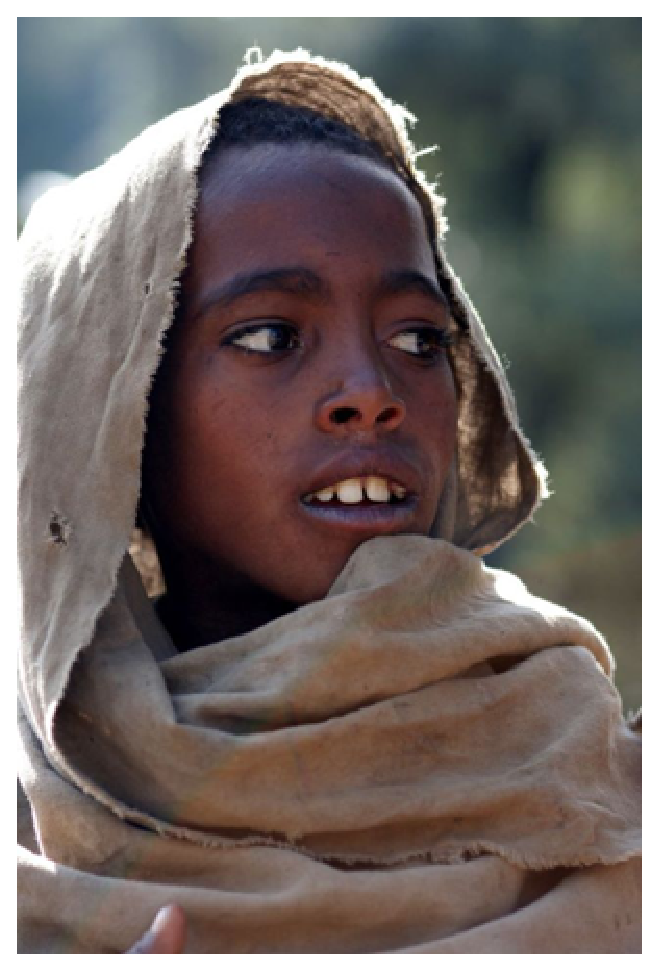
\includegraphics{etiopan.eps}}
                        \reflectbox{\scalebox{0.45}{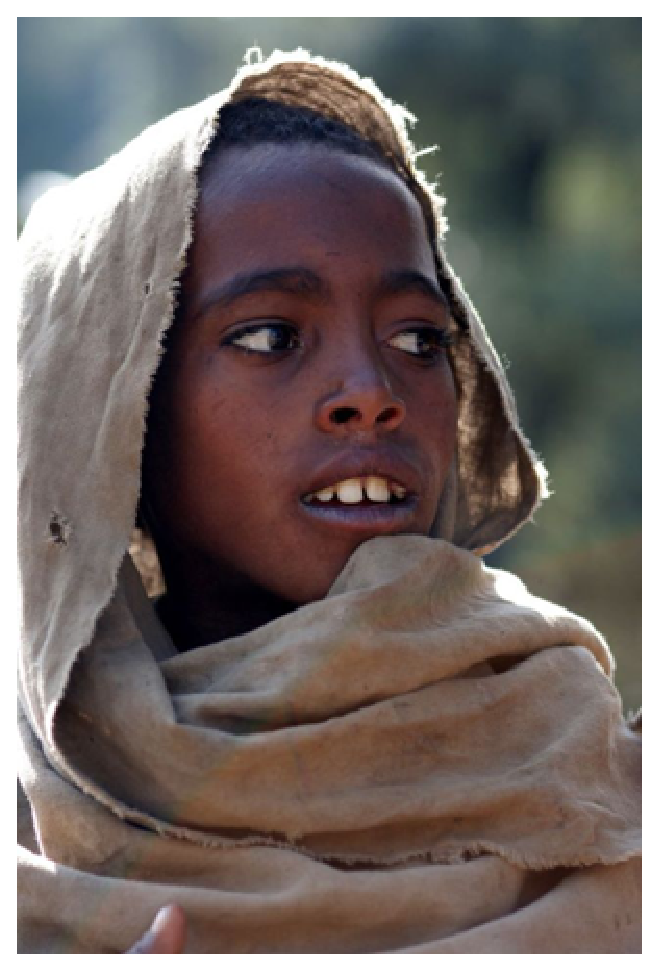
\includegraphics{etiopan.eps}}}
                        \caption{Malý Etiopánek a~jeho bratříček}
                        \label{Etiopanek}
                \end{figure}

                Rozdíl mezi vektorovým \dots
                \begin{figure}[h]
                    \centering
                    \scalebox{0.45}{
\includegraphics{oniisan.eps}}
                    \caption{Vektorový obrázek}
                    \label{OniisanVec}
                \end{figure}

                \dots a~bitmapovým obrázkem
                \begin{figure}[h]
                    \centering
                    \scalebox{0.7}{
\includegraphics{oniisan2.eps}}
                    \caption{bitmapový obrázek}
                    \label{OniisanBit}
                \end{figure}\\
                se projeví například při zvětšení.

                Odkazy (nejen ty) na~obrázky~\ref{Etiopanek}, \ref{OniisanVec} a~\ref{OniisanBit}, na tabulky \ref{Kurzy}~a~\ref{KleenehoTab}~a také na~algoritmus \ref{FastSLAM} jsou dělány pomocí křížových odkazů. Pak je ovšem potřeba zdrojový soubor přeložit dvakrát.

                Vektorové obrázky lze vytvořit i přímo v~\LaTeX u, například pomocí prostředí \verb|picture|.

                

                \newpage
                \begin{landscape}
                    \begin{figure}
                       
                    \linethickness{2pt}
                    \framebox(650,400){
                        
                        \begin{picture}(500,350)
                            \linethickness{4pt}
                        \put(20,0){\line(1,0){460}} % base
                            \linethickness{1pt}
                        \put(50,0){\line(0,1){100}} % l-wall
                        \put(450,0){\line(0,1){100}} % r-wall
                        \put(50,100){\line(1,0){400}} % strop
                        \put(200,0){\line(0,1){100}} % garaz
                        \put(70,0){\line(0,1){80}} % l-vrata
                        \put(180,0){\line(0,1){80}} % r-vrata
                        \put(70,80){\line(1,0){110}} % hor-vrata
                        \put(70,60){\line(1,0){110}} % lamela-vrataI
                        \put(70,40){\line(1,0){110}} % lamela-vrataII
                        \put(70,20){\line(1,0){110}} % lamela-vrataIII
                        \put(50,100){\line(1,1){70}} % l-strecha
                        \put(450,100){\line(-1,1){70}} % r-strecha
                        \put(120,170){\line(1,0){260}} % strop
                        \put(320,170){\line(0,1){20}} % r-komin
                        \put(300,170){\line(0,1){20}} % l-komin
                        \put(300,190){\line(1,0){20}} % up-komin
                        \put(215,0){\line(0,1){70}} % l-dvere
                        \put(260,0){\line(0,1){70}} % r-dvere
                        \put(215,70){\line(1,0){45}} % hor-dvere
                        \put(225,35){\oval(12,5)[l-left]}    %klika 
                        \put(290,30){\line(0,1){40}} % l-okno
                        \put(340,30){\line(0,1){40}} % r-okno
                        \put(290,70){\line(1,0){50}} % hor-okno
                        \put(290,30){\line(1,0){50}} % dol-okno
                        \put(360,30){\line(0,1){40}} % l-oknoII
                        \put(410,30){\line(0,1){40}} % r-oknoII
                        \put(360,70){\line(1,0){50}} % hor-oknoII
                        \put(360,30){\line(1,0){50}} % dol-oknoII
                        \put(480,300){\circle{40}} % dol-oknoII
                    \end{picture}
                    }
                    \caption{Vektorový obrázek moderního bydlení vhodného pro 21. století. (Buďto vytvořte stejný obrázek, anebo nakreslete pomocí \texttt{picture} váš vlastní domov.)}
                \end{figure}
                \end{landscape}

\end{document}